\section{Convolution Neural Network Utilization}

First, we describe how to use a convolutional network for parsing result processing. Parsing result is a boolean matrix and we utilize the artificial neural network to detect sufficient features and find patterns in their appearance.
Therefore, we need to transform these boolean matrices to some data structure acceptable by the neural network: vector or image.
Currently, we came up with two possible ways.

The first one is to drop out the nullary bottom left triangle, vectorize the top right triangle row by row and transform it into a byte vector.
This approach reduces the input size, but it requires all the input sequences to have equal length.
Thus we propose to either cut sequences to be of some predefined length or to pad them up with some blank symbols.
Vectorization breaks data locality which makes learning harder: the network should restore back the relations broken during linearization.
This also means that learning takes more time.

The second way is to represent the matrix as an image: the false bits of the matrix as white pixels and the true bits as black ones.
This approach makes it possible to process sequences of different lengths since the images are easily transformed to a specified size.
Data locality is also preserved: the information about relative positions of extracted basic features does not get lost which should improve learning.

The architecture of the neural network that takes vectorized data as an input is described in~\cite{grigorevcomposition} and it consists of the long sequence of interchangeable dense and dropout layers with aggressive batch normalization. 
To handle images, we propose to use a network which consists of a small number of convolutional layers, linearization, and dense network which has a similar architecture as for vectorized data.
An example of proposed architecture id provided in figure~\ref{nn} (network \textbf{\texttt{N1}}).

\section{Parsing Step Elimination}

Another improvement that we came up with concerns parsing elimination in the context of our solution. 
The idea is to create a model which can handle original sequences instead of the parsing matrices. For that, we propose to use two-staged learning: first, a network which solves a subtask is trained and then it is used as pretrained layers in the training of the resulting network.
In our solution, we first train a neural network to handle parsing results which performs classification according to a problem at hands. We create two networks in order to compare different architectures: one of them handles vectorized parsing result, the other handles parsing result represented as a bitmap image. After that, we extend these neural networks by several input layers that take the initial nucleotide sequence as an input and convert it to the parsing result which is handled appropriately by the pretrained layers.

Figure~\ref{nn} represents the detailed description of these three neural networks architectures.
Here \textbf{\texttt{N1}} is a network which handles images, \textbf{\texttt{N2}} is a network which handles vectorized parsing results, and \textbf{\texttt{N0}} is an additional block which converts the input sequence into a set of features which can be handled by using \textbf{\texttt{N1}} or \textbf{\texttt{N2}}. So, firstly we train \textbf{\texttt{N1}} and \textbf{\texttt{N2}} on parsed data. After that, for vector-based network we combine the extension \textbf{\texttt{N0}} and the whole original sequence of layers and for image-based network we use the similar architecture, except we remove the convolutional layer from the extended model, thus, the first layer at the junction of the blocks corresponds to the linearized image.

\begin{figure}[h]
\begin{center}
\centering
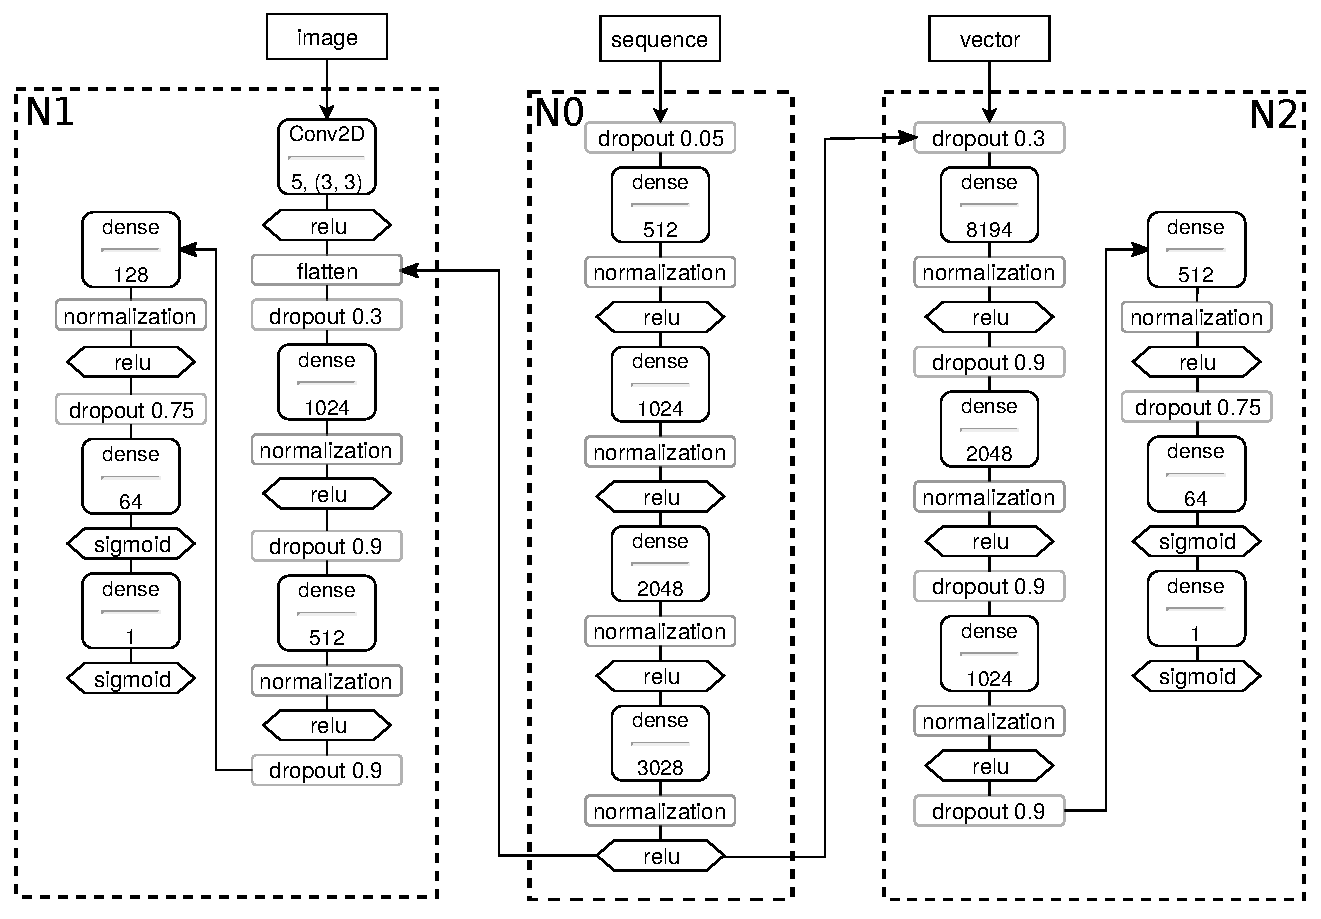
\includegraphics[width=12cm]{figures/nn_arch.pdf}
\caption{Neural networks architectures}
\label{nn}
\end{center}
\end{figure}

To sum up, we developed a technique to process parsing matrices as images by convolutional neural networks. 
Also, we built a model that handles sequences and requires parsing only for training the network it is based on. 
This removes the parsing step from the usage of the trained model.
